\documentclass{article}
\usepackage[top=2.54cm, bottom=2.54cm, left=2.54cm, right=2.54cm]{geometry}
\usepackage{graphicx,color,url,amsmath}
\usepackage{enumerate}
\setlength{\parskip}{12pt}
\setlength{\parindent}{0pt}
\begin{document}

\begin{center} Huilin Tong\\
ID:1261574
\end{center}

{\bf Discussion}\\

\begin{enumerate}
\item Yes, the answer is exactly the same as HW1.
\item Since the age differences of each age group is large, it's more accuracy to keep tracking in every one year's gruop.
\item The total population increased after 5 years according to the model.
\item Total population will decrease if not taking young juveniles into account.
\item Model is conducted under ideal situation. But in actual environment, maybe temperature is extremely hot this year than before or it's too dry without any rainfall will all lead to a sharp decrease in turtle population. Or maybe a sudden species invasion also will decrease the population. While the model still correct if keep everything the same as the data used in building the model.
	
\end{enumerate}

{\bf Extra credit}\\
By increasing the given vital rate by $5\%$ in each age group separately, two years loop of different shown in the below figure. Clearly, increasing the survival rate in older adults is the most effectively as it enjoys the fastest growth in total population. 


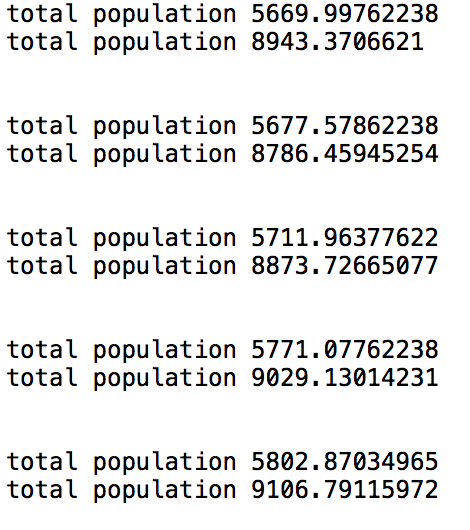
\includegraphics[scale=0.6]{EC.png}	



\end{document}